Results...

\subsection{Experiment Results}


% \subsection{Synthetic model evaluation}

\subsubsection{Local interpretation methods comparison}
As was pointed out before, in this experiment, the Breast Cancer dataset was examined. After exploring the dataset, it was noticed that the attribute “area\_mean” was one of the most important features according to the permutation feature importance ranking. Without loss of generality, we could randomly choose one instance and try to provide reasonable explanations. In this scenario, we decided to choose instance 10 from the dataset, and the boosting algorithm was utilized to train a black box model. Therefore, the following results were demonstrated based on the experiment that was intended to inspect the variable “area\_mean” in an ensemble model on the processed dataset. 

First local interpretation approach was numeric perturbation, which was applicable only to numeric attribute. The assumption was that we already had the black box model and the selected instance being explained. It could be easily estimated that there was 89% chance to be predicted as a malignant cancer. Nonetheless, if we deviated the “are_mean” value of the instance by one positive and negative standard value, the probability would increase 0.5% and decrease 65% respectively. In a sense, we could argue that this attribute played a critical role when making predictions. 

The next local interpretation method was LIME. After selecting the instance of interest, it was required to generate neighborhood points by perturbing the instance. To be more specific, the neighborhood points were produced by sampling from Normal(0, 1), multiplying by the standard deviation and adding back the mean value. Then, a weighted intrinsic interpretable model was fitted to explain the prediction making by the classifier. In this way, the model was supposed to be locally faithful around the explained instance. As displayed in Fig~\ref{fig:breast_lime}, the classifier determined that the cancer was malignant with probability 0.89. It could be noticed that features, such as “area\_mean” or “texture\_mean”, had huge impact on the prediction due to the large coefficient in the model. Note that this approach would discretize numerical feature values into quartiles. For instance, it was observed that when the condition “area\_mean > 0.27” was met, the weight for this feature was 0.35. It could be interpreted that if we decreased one unit on this feature value, the chance of the cancer to be malignant would decline 0.35. And on the right side, the feature value pairs of the instance to be explained was displayed in a table format. The feature columns showed the feature names and the value column displayed the original value for the corresponding feature. 

\begin{figure}[H]
	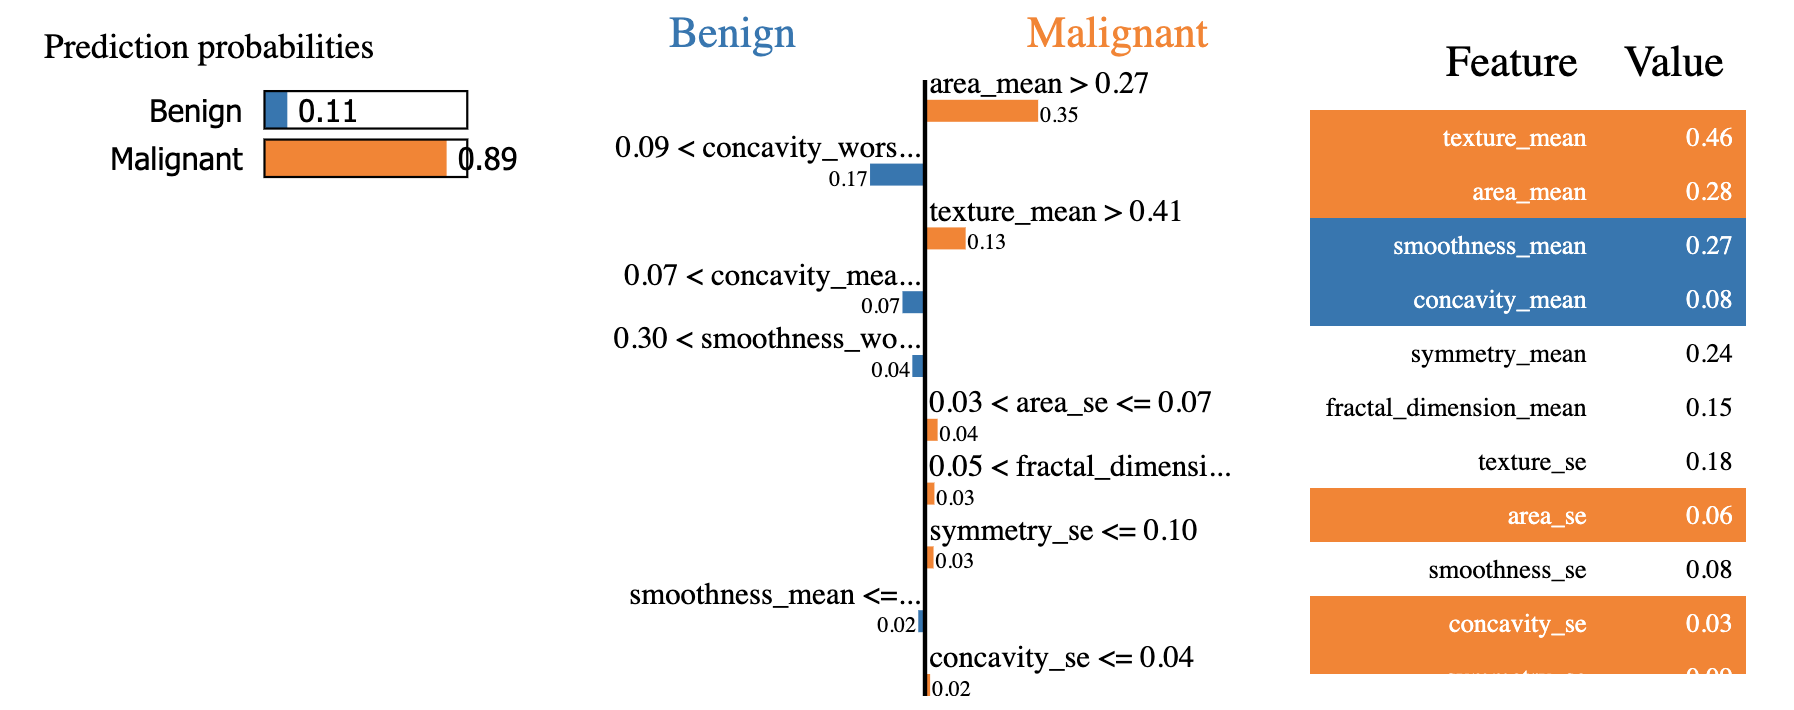
\includegraphics[width=0.9\textwidth]{imgs/breast_lime_plot.png}
	\caption{On the left side, the prediction probabilities were shown, telling that the tumor had 89\% chance to be predicted as malignant. In the middle, the feature weights in the fitted model were  displayed. In particular, the weight for attribute “area\_mean” is 0.35. Note that the feature value pair of the instance being explained were listed on the right side.}
	\label{fig:breast_lime}
\end{figure}

Another local explanation method that we adopted was Kernel SHAP. Nonetheless, despite the fact that the back box model here we trained was tree ensemble model, the more efficient TreeSHAP estimation could be used instead. By applying this approach, it was aimed to compute shapley values for each feature, which were regarded as the feature contributions. As depicted in Fig~\ref{fig:breast_shap} , it gave a nice reasoning which showed feature influence on this prediction. The shapley value could be visualized as “forces” and each feature value was a force either increased or decreased the prediction. As was seen, there was a base value denoted as -1.44, which was the average model output over all predictions. The below explanation showed features each contributing to push the model output from the base value to the actual model output. Features pushing the prediction higher were shown in red, those pushing the prediction lower were in blue. The shapley value for each feature was attached in the figure, but it had to be noted that by default the shapley value were displayed in the logit space and all those shapley values summed up to the difference between the model output for that instance and the expected base value. Therefore, we could infer that for this instance, attributes “area\_mean” and “area\_se” had a dominant effect on the prediction, while “concavity\_worst” had reverse impact. 

\begin{figure}[H]
	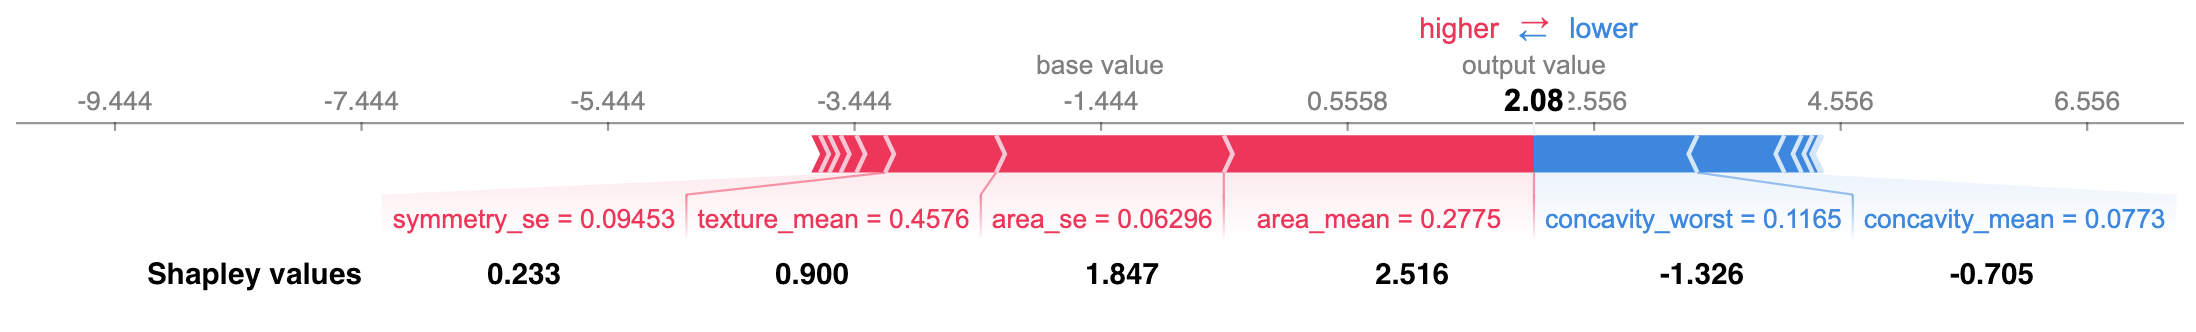
\includegraphics[width=0.9\textwidth]{imgs/breast_shap_force_plot.png}
	\caption{SHAP values to explain the influence of features leading to the prediction of benign or malignant cancer. The base value was the average probability over all predictions in logit space, which was -1.44. Shapley values were attached for each feature value as well. Feature values shown in red had positive effect in increasing the risk of being malignant cancer, while feature values denoted in blue declined the probability.}
	\label{fig:breast_shap}
\end{figure}

\subsubsection{Decision tree vs. Subgroup discovery}

Given the fact that both decision tree algorithm and subgroup discovery technique could be used to discover hidden pattern in data with respect to the effect of a specific attribute, it could be interesting to have a comparison. In this experiment, we decided to choose German Credit dataset, with the aim to predict whether a person has a good or bad credit risk. Since this dataset contained multivariate attributes, the dataset was processed by dummy encoding in this scenario. After exploring the dataset, the attribute “Credit amount” was selected to inspect the effect in the dataset. Thus, the first step was to measure the impact of feature “Credit amount” in each individual instance. In principle, all those aforementioned local interpretation methods supported the feature effect measurement. Nevertheless, Kernel SHAP approach was finally chosen. Following this approach, the shapley value of attribute “Credit amount” was computed for each instance. 

By taking the shapley values as the target, it was assumed that local patterns could describe the influence of the selected attribute in the dataset. In this case, a tree-like graph could be drawn based on the decision tree algorithm. It had to be noticed that the maximal tree depth was set to three. As demonstrated in Fig~\ref{fig:credit_decision_tree}, the first splitting node was “Purpose=furniture/equipment”. By following the rightmost path, it led us to a pattern with high value, meaning that the attribute “Credit amount” revealed a significant impact on the dataset complied with this pattern. This pattern could be described as “Purpose=furniture/equipment AND Duration >13.5 AND Age > 31.5”. 

\begin{figure}[H]
	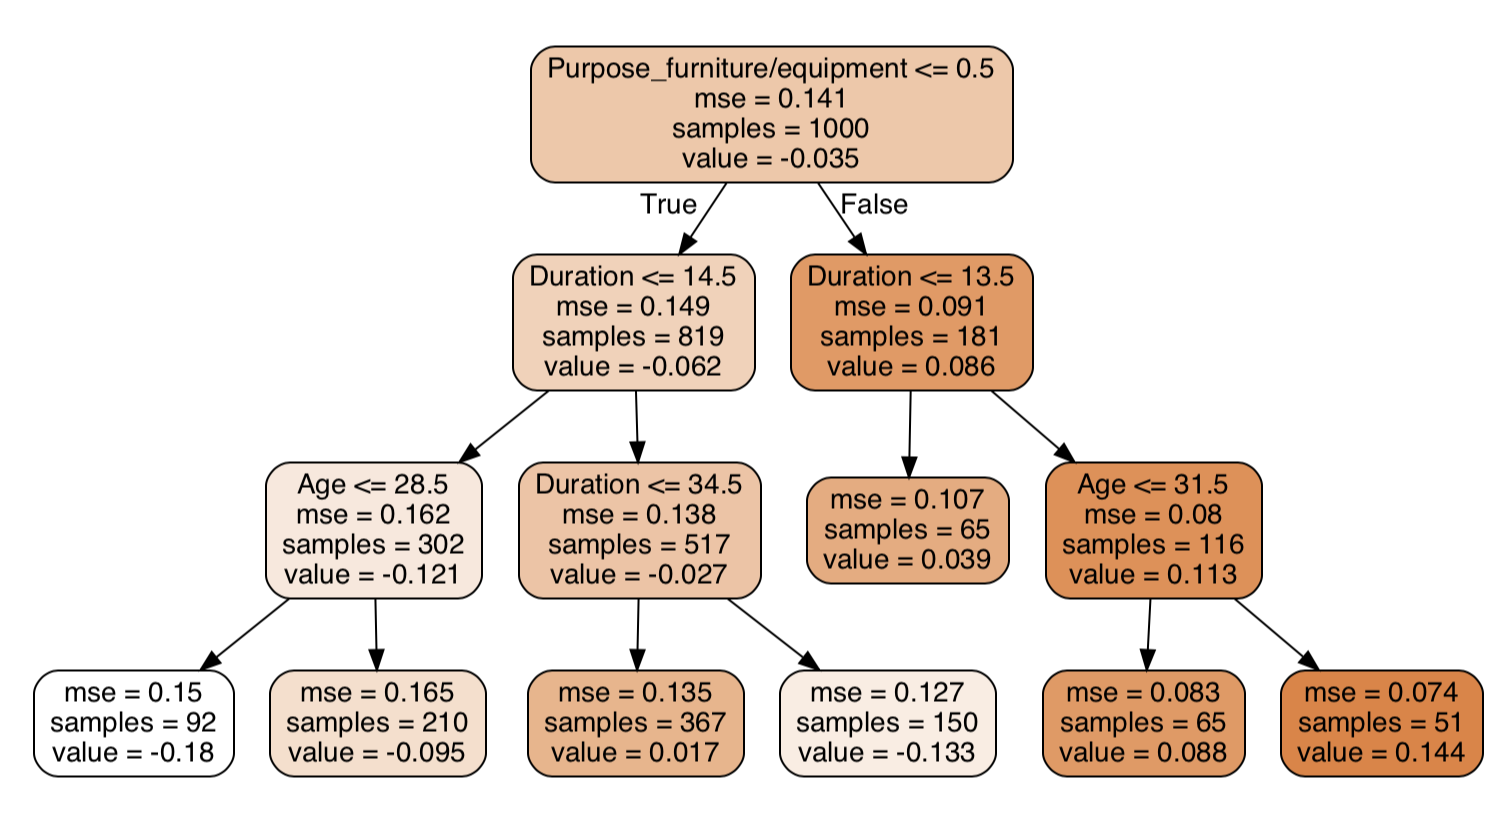
\includegraphics[width=0.9\textwidth]{imgs/credit_decision_tree.png}
	\caption{Decision tree}
	\label{fig:credit_decision_tree}
\end{figure}

In contrast, by considering the shapley value as the numeric target in subgroup discovery technique, those interesting subgroups could be found out as shown in Table~\ref{fig:credit_subgroup}. As could be seen, the average shapley value over the entire dataset was about -0.03, while this value was 0.08 in the subgroup “Purpose=furniture/equipment”, which also corresponded to the first splitting node. And the patterns “Duration >13.5” and “Age > 31.5” depicted in the path along the decision tree was also covered by the discovered subgroups in the table. 

\begin{figure}[H]
	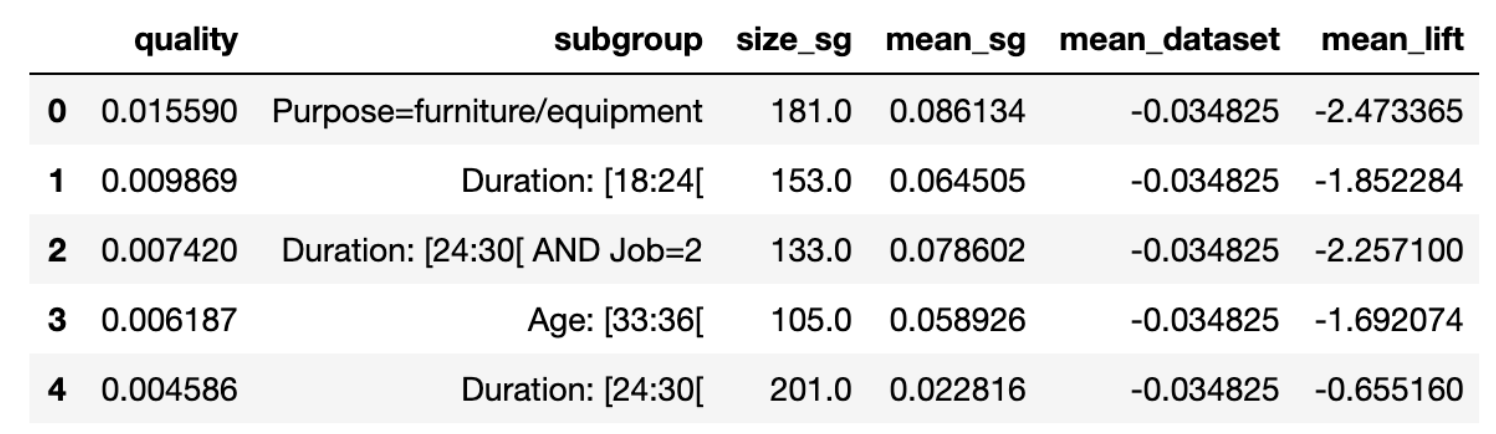
\includegraphics[width=0.9\textwidth]{imgs/credit_subgroup.png}
	\caption{Subgroup discovery results}
	\label{fig:credit_subgroup}
\end{figure}

Considering the similar patterns discovered by both techniques, we might argue that there indeed existed some patterns that the feature had a significant impact, and further influenced the model prediction.

\subsubsection{Case study} 
As clarified in the last chapter, the first case study was experimented on the Adult Income dataset. The task for the experiment was to interpret the influence of a specific attribute in a black box model, and we assumed that the dataset and the model was provided. Initially, the dataset was processed as before by encoding the data and removing correlated features. Afterwards we randomly split the dataset into training set and testing set, and a simple full-connected neural network was trained based on the training data. By far, we had the neural network model and testing data, and the next step was to find out impact of a particular feature in a single instance. Furthermore, we were asked to discover some subgroups where the inspected feature had a dominant influence. 

At the beginning, the importance of each feature was explored, which gave an indication about features that were worthy of attention. Apart from the permutation feature importance approach to estimate the importance degree of each feature, an alternative method to measure the importance was based on the magnitude of feature contributions using shapley values, called SHAP feature importance measure. The intuition was that features with large mean absolute shapley values were important. From the Fig~\ref{fig:adult_bar}, we could tell that “age” was the most important feature comparative to others. Considering that we would like to further compare the pattern mining results based on the feature effects calculated by binary flip approach and kernel SHAP approach, the attribute “sex” was chosen to explore since the binary flip method was designed for exploiting the  binary feature. 

\begin{figure}[H]
	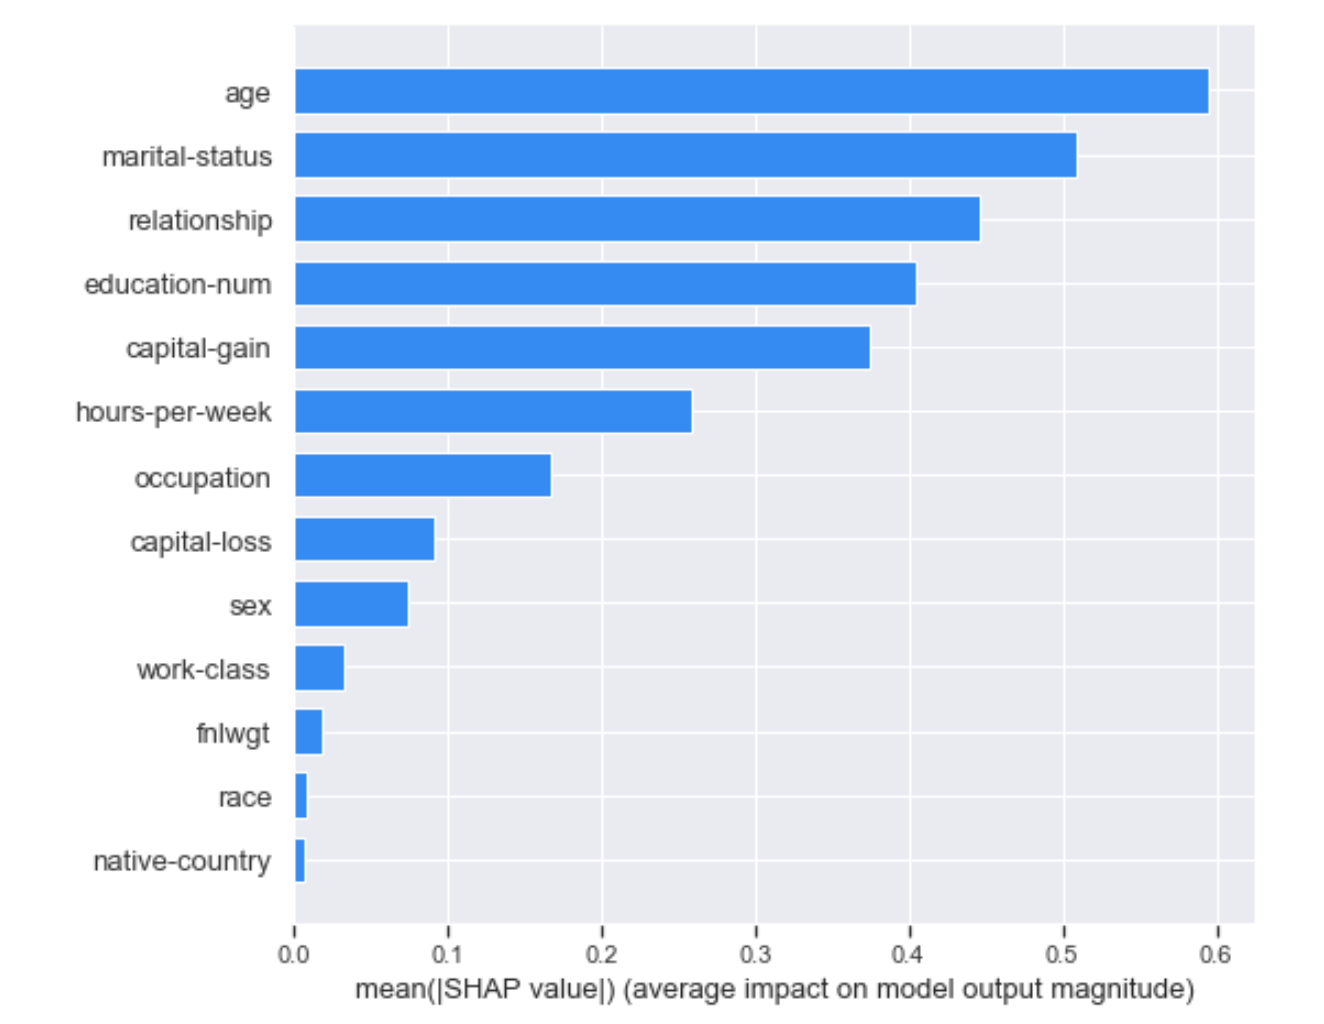
\includegraphics[width=0.9\textwidth]{imgs/adult_bar_plot.png}
	\caption{SHAP feature importance measure was based on the magnitude of feature contributions, and it was assessed by the mean absolute shapley values. “Age” was the most important feature.}
	\label{fig:adult_bar}
\end{figure}

From binary flip method, we could obtain the effect when changing the sex for each instance by calculating the prediction change. As for the kernel SHAP approach, the effect of sex was estimated by this feature contribution by computing the shapley values. Then subgroup discovery technique was applied to the dataset while taking the effect of sex as the target. Therefore, two different results were combined with respect to two different measurements and they were displayed in Table~\ref{fig:adult_subgroup}. Each part represented the interesting subgroups that were discovered. From Table~\ref{fig:adult_subgroup}, it was noticed that these two results were similar in some degree. For instance, they both discovered the pattern such as “relationship=Husband” and “marital-status=Married-civ-spouse”. 

\begin{figure}[H]
	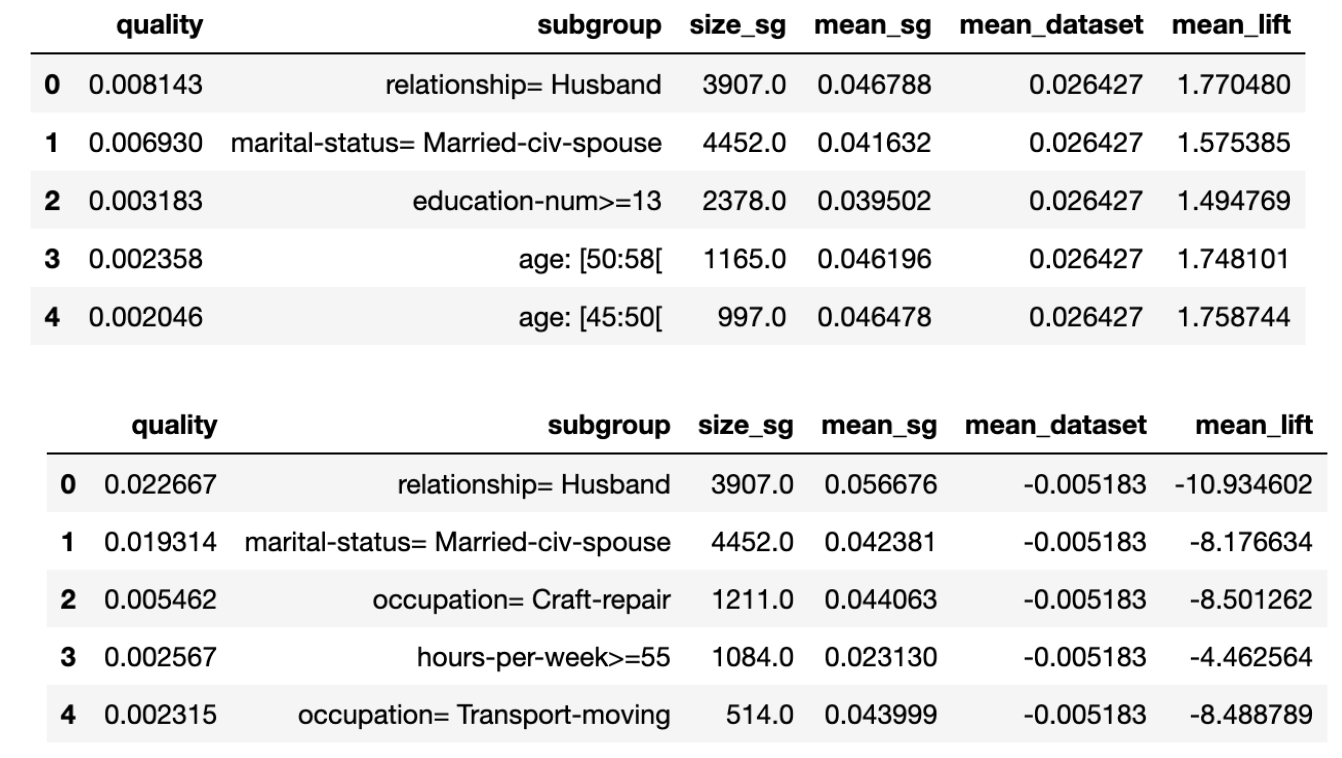
\includegraphics[width=0.9\textwidth]{imgs/adult_subgroup.png}
	\caption{Subgroup discovery results}
	\label{fig:adult_subgroup}
\end{figure}

It could be concluded that there were patterns in data that feature “sex” had a huge impact no matter what local interpretation methods were used. 
